% This is "sig-alternate.tex" V2.0 May 2012
% This file should be compiled with V2.5 of "sig-alternate.cls" May 2012
%
% This example file demonstrates the use of the 'sig-alternate.cls'
% V2.5 LaTeX2e document class file. It is for those submitting
% articles to ACM Conference Proceedings WHO DO NOT WISH TO
% STRICTLY ADHERE TO THE SIGS (PUBS-BOARD-ENDORSED) STYLE.
% The 'sig-alternate.cls' file will produce a similar-looking,
% albeit, 'tighter' paper resulting in, invariably, fewer pages.
%
% ----------------------------------------------------------------------------------------------------------------
% This .tex file (and associated .cls V2.5) produces:
%       1) The Permission Statement
%       2) The Conference (location) Info information
%       3) The Copyright Line with ACM data
%       4) NO page numbers
%
% as against the acm_proc_article-sp.cls file which
% DOES NOT produce 1) thru' 3) above.
%
% Using 'sig-alternate.cls' you have control, however, from within
% the source .tex file, over both the CopyrightYear
% (defaulted to 200X) and the ACM Copyright Data
% (defaulted to X-XXXXX-XX-X/XX/XX).
% e.g.
% \CopyrightYear{2007} will cause 2007 to appear in the copyright line.
% \crdata{0-12345-67-8/90/12} will cause 0-12345-67-8/90/12 to appear in the copyright line.
%
% ---------------------------------------------------------------------------------------------------------------
% This .tex source is an example which *does* use
% the .bib file (from which the .bbl file % is produced).
% REMEMBER HOWEVER: After having produced the .bbl file,
% and prior to final submission, you *NEED* to 'insert'
% your .bbl file into your source .tex file so as to provide
% ONE 'self-contained' source file.
%
% ================= IF YOU HAVE QUESTIONS =======================
% Questions regarding the SIGS styles, SIGS policies and
% procedures, Conferences etc. should be sent to
% Adrienne Griscti (griscti@acm.org)
%
% Technical questions _only_ to
% Gerald Murray (murray@hq.acm.org)
% ===============================================================
%
% For tracking purposes - this is V2.0 - May 2012

\documentclass{sig-alternate}
\usepackage{pygmentize}
\usepackage{minted}
\usepackage{graphicx}
\usepackage{xcolor,listings}
\usepackage{textcomp}
\lstset{upquote=true}

\begin{document}
%
% --- Author Metadata here ---
\conferenceinfo{Data For Good Exchange, 2015}\\

\title{Optimizing Local Smoke Alarm Inspections\\with Federal Data}
%
% You need the command \numberofauthors to handle the 'placement
% and alignment' of the authors beneath the title.
%
% For aesthetic reasons, we recommend 'three authors at a time'
% i.e. three 'name/affiliation blocks' be placed beneath the title.
%
% NOTE: You are NOT restricted in how many 'rows' of
% "name/affiliations" may appear. We just ask that you restrict
% the number of 'columns' to three.
%
% Because of the available 'opening page real-estate'
% we ask you to refrain from putting more than six authors
% (two rows with three columns) beneath the article title.
% More than six makes the first-page appear very cluttered indeed.
%
% Use the \alignauthor commands to handle the names
% and affiliations for an 'aesthetic maximum' of six authors.
% Add names, affiliations, addresses for
% the seventh etc. author(s) as the argument for the
% \additionalauthors command.
% These 'additional authors' will be output/set for you
% without further effort on your part as the last section in
% the body of your article BEFORE References or any Appendices.

\numberofauthors{3} %  in this sample file, there are a *total*
% of EIGHT authors. SIX appear on the 'first-page' (for formatting
% reasons) and the remaining two appear in the \additionalauthors section.
%
\author{
% You can go ahead and credit any number of authors here,
% e.g. one 'row of three' or two rows (consisting of one row of three
% and a second row of one, two or three).
%
% The command \alignauthor (no curly braces needed) should
% precede each author name, affiliation/snail-mail address and
% e-mail address. Additionally, tag each line of
% affiliation/address with \affaddr, and tag the
% e-mail address with \email.
%
\alignauthor
Marc DaCosta\\
       \affaddr{Co-founder, Enigma}\\
       \email{marc@enigma.io}
\alignauthor
Jeremy Krinsley\\
       \affaddr{Engineer, Enigma}\\
       \email{jak@enigma.io}
\alignauthor
Brian Abelson\\
       \affaddr{Engineer, Enigma}\\
       \email{brian@enigma.io}
}

\maketitle
\begin{abstract}
This paper outlines a fully-realized civic tool that predicts municipal blocks least likely to have homes with functioning smoke alarms and most likely to have residents who are at highest risk for fire fatality. Using a novel merge of the American Community Survey (ACS) and the American Housing Survey (AHS), we are able to model these two risk factors at the geography of census block groups, and with the aid of the TIGER Census dataset, return actual street addresses with associated risk scores. This tool represents a potential model for developing reusable civic analytic applications that can serve multiple cities while responding to local particularities.
\end{abstract}

\keywords{Civic Analytics, Fire Prevention, Census, ACS, AHS, TIGER }


\section{Intro}
We can expect 20,000 people to be injured or killed by fires in the United States this year. With over 130 million housing units across the country, 4.5 million of them do not have smoke detectors, placing their inhabitants at substantial risk. Driving this number down is the single most important factor for saving lives put at risk by fire.

A broad range of people are trying to address this problem, from local fire departments to the Red Cross. However, they all face the same problem: What door do we knock on first?

A community knows best which blocks and which citizens are at risk for injury or death in a fire. First responders and outreach organizations know the facts of their municipality better than a dataset ever can: firemen know their districts; Red Cross volunteers and religious organizations know their local residents. These are the instincts that up to now have been the primary, if not the only resources available to identify at-risk homes and residents. 

With that in mind, we have gone farther than any previous effort to rank likelihood of smoke alarm risk by city block in the hopes that our work can offer more precise and granular leads for those who perhaps had no such prior resources. What we are able to present is a systematic ranking by city block for 209 cities that fall within 40 census-tabulated Metropolitan Statistical Areas (MSAs). We have furthermore developed a tool that allows these same first responders and active community members to improve the accuracy of local scores by uploading fire data via an API into our model.

\section{Background}

In November of 2014 there was a house fire in the Broadmoor neighborhood of New Orleans, killing five people, including three children. The house did not have a smoke alarm in it. Enigma began working with New Orleans' Fire Department and Office of Performance and Accountability to develop a model that identified New Orleans blocks least likely to have smoke alarms, and most likely to experience a fire fatality. This enabled the New Orleans Fire Department to conduct a door-to-door outreach campaign to place smoke alarms in as many at risk homes as possible. Drawing on the learnings from New Orleans, we extended the model to apply to the entire United States, in hopes that more people can use and improve on our insights.


\section{Components}

The risk model and resulting tools were built off of a number of different federal census datasets. Below we outline these datasets and the ways in which we used them. We are also releasing all of the data components and algorithms that make this tool work, in hopes that others can improve upon what we have begun.

\subsection{AHS/ACS Merge}

The central crux of our work employs a systematic join of the American Housing Survey (AHS), a resource for nationally-representative, detailed housing characteristics, and the American Community Survey (ACS)\footnote{https://github.com/enigma-io/ahs-acs}, the census' most extensive and thorough demographic survey. This merge generates meaningful local data from a federal dataset that was once used only to describe characteristics normalized at the level of entire cities.

Making the ACS-AHS merge a machine-readable process greatly enhances the value of the data in the AHS, and by extension, enriches what we can learn about a given few blocks within the biggest metro-areas in the U.S. We are not the first\footnote{http://www.census.gov/content/dam/Census/programs-surveys/ahs/publications/CombiningAHS-ACS.pdf} to attempt a method for explaining the relationship between the two datasets. However, to the best of our knowledge, we have gone the furthest in making that process programmatic and fully machine-readable.

Many questions asked in the AHS directly mirror those asked in the ACS. For instance, both surveys ask about a respondent's age. While the ACS groups these responses into bucketed counts per block group (i.e. "Males under the age of 5" or "Females between the ages of 70 and 74"), the AHS simply records the respondent's actual age (4 or 72). While both surveys capture the same concept, they each record this information in different ways. Our merge enables translations between the two surveys by mapping these concepts into a common schema. This is useful as it allows models trained on AHS data to be scored on ACS data. 

We came up with these mappings by scanning the AHS Codebook for questions that were also asked in the ACS. For the most part, these were demographic variables and information about a respondent's household. In the case of the AHS, responses are recorded in categories (i.e. "married" = 3 and "divorce" = 4), or continuous numbers ("year house built" = 1964). On the other hand, as mentioned above, the ACS buckets responses by counts for census geographies, like block groups and tracts. In order to map the two surveys, we had to similarly bucket AHS responses into binary indicators. Here's an example of what this process looks like for "Marital Status":
\begin{minted}[
	frame=none,
	breaklines=true
]{yaml}
- concept: Marital Status 
  ahs:
        type: categorical
        var: hhmar 
        map:
            hhmar_married_spouse_present: 1
            hhmar_married_spouse_absent: 2
            hhmar_widowed: 3
            hhmar_divorced: 4
            hhmar_separated: 5
            hhmar_never_married:  6

  acs:
        table: B12001
        total: B12001001
        map:
            hhmar_married_spouse_present: [B12001005,B12001014]
            hhmar_married_spouse_absent: [B12001006, B12001015]
            hhmar_widowed: [B12001009, B12001018]
            hhmar_divorced: [B12001010, B12001019]
            hhmar_separated: [B12001007, B12001016]
            hhmar_never_married: [B12001003, B12001012]
\end{minted}

\subsection{Risk Model}

Armed with this novel dataset, we set about to develop a model to estimate the risk that residents of a particular census block group risk lack a smoke alarm.  An outline of our approach is as follows:

\begin{enumerate} 
\item Leverage exploratory analysis to select an appropriate sample from the AHS.
\item Train a national-level logistic regression on the AHS.
\item Train one logistic regression for each MSA in the AHS with an added model weighting function.
\item Compute scores for the national and MSA-level models and merge based on MSA model weight.
\end{enumerate}

\subsubsection{Handling Missing Data in the AHS}

The AHS does not require that subjects respond to all questions. As a result, there's a lot of missing data. We deal with this problem via the following steps:

\begin{figure}
\centering 
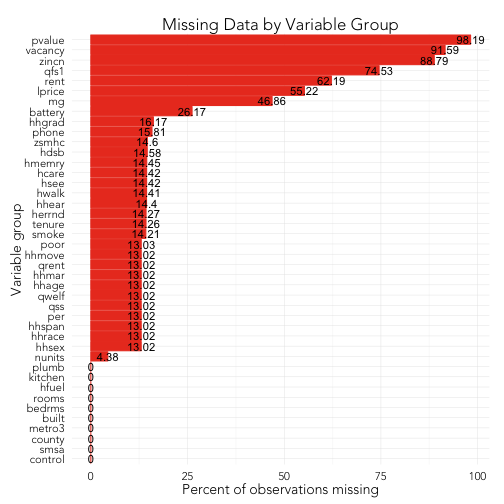
\includegraphics[scale=0.42]{missing-data-1.png}
\caption{Missing data in the AHS by variable group}
\end{figure}

\begin{enumerate} 
\item Drop all observations with greater than 90\% of missing variables. 
\item Drop all observations with a missing dependent variable.
\item Drop all variable groups with greater than 50\% of missing data (Figure 1).
\item Randomly impute missing data by sampling from it's existing distribution.
\end{enumerate}

Out of the 186448 rows in the AHS, we were able to keep 155108 rows through this process, or 83.2\% of the total. 

\subsubsection{Covariate Selection}

Through a simple correlation analysis, we settled on number of variable groups to model in the AHS:

\begin{itemize} 
\item ``built'' - The year the household was built. 
\item ``poor'' - Percentage of income relative to the poverty level. observations with a missing dependent variable.
\item ``hhmove'' - The year the current resident moved in.
\item ``hhgrad'' - The eduction level of the homeowner.
\item ``hhrace'' - The race of the homeowner.
\item ``hhspan'' - Whether the homeowner is of hispanic descent.
\item ``hfuel'' - The type of fuel the home uses for heating. 
\item ``tenure'' - The rental status of the homeowner.
\item ``mg'' - The mortgage status of the homeowner.
\end{itemize}

\begin{figure}
\centering 
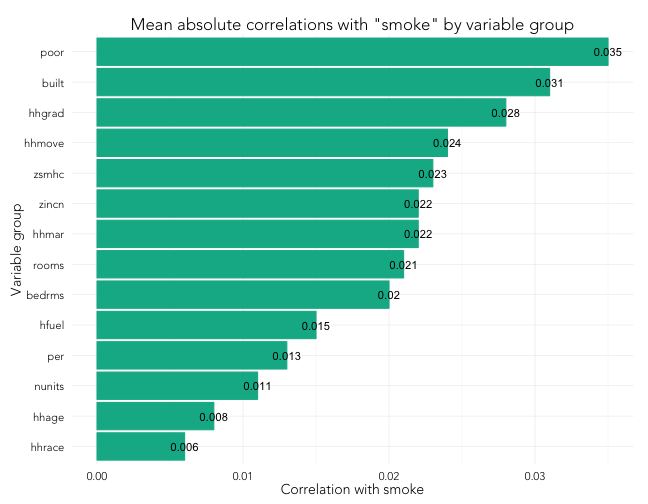
\includegraphics[scale=0.42]{explore-correlations-1-2.png}
\caption{Mean absolute correlations with "smoke" by variable group}
\end{figure}

These groups translated into the following model (written in R syntax):

\begin{minted}[
	frame=none,
	breaklines=true
]{r}
# our model's formula
f <- smoke ~  
       built_1980_to_1989 +
       built_1960_to_1969 +
       built_2010_to_later +
       built_1990_to_1999 +
       built_1950_to_1959 +
       built_1939_or_earlier +
       poor_50_to_99 +
       poor_under_50  +
       poor_184_to_199 +
       poor_125_to_149 +
       poor_100_to_124 +
       poor_150_to_184 +
       hhmove_moved_in_1990_to_1999 +
       hhmove_moved_in_1969_or_earlier +
       hhmove_moved_in_2000_to_2009 +
       hhmove_moved_in_1970_to_1979 +
       hhmove_moved_in_1980_to_1989 +
       hhgrad_associates_degree +
       hhgrad_7th_or_8th_grade +
       hhgrad_9th_grade +
       hhgrad_doctorate_degree +
       hhgrad_5th_or_6th_grade +
       hhgrad_regular_high_school_grad +
       hhgrad_bachelors_degree +
       hhgrad_1st_2nd_3rd_4th_grade +
       hhgrad_11th_grade +
       hhgrad_less_than_1st_grade  +
       hhgrad_12th_grade_no_diploma +
       hhrace_hawaiian_pac_isl_only +
       hhrace_asian_only +
       hhrace_other +
       hhrace_black_only +
       hhrace_native_am_only +
       hhrace_white_only +
       hhspan_yes +
       tenure_renter_occupied +
       hfuel_wood +
       mg_yes
\end{minted}

\subsubsection{National Model}

First, we estimate national-level coefficients by training a logistic regression with the above formula on the entirety of our AHS sample.

Only 4\% of respondents answered negatively to the question "Do you have a working smoke alarm?" For such rare events, it can be difficult to generate robust coefficients. We deal with this issue by bootstrapping the coefficients and artificially inflating the distribution of negative respondents for each iteration. Our final coefficients are the median of all the coefficients generated from 1000 iterations (Figure 3). The national-level model suggests that  people who didn't have smoke alarms tended to be uneducated, hispanic, not have mortgages, and live in older homes.

\begin{figure}
\centering 
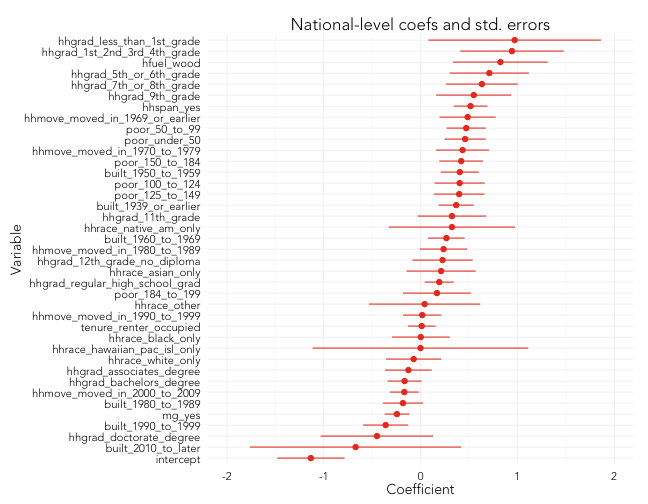
\includegraphics[scale=0.36]{generate-model-2.png}
\caption{Bootstrapped. National-level coefficients and std. errors.}
\end{figure}

\subsubsection{MSA Models}
We estimate MSA-level coefficients by training identical models for each MSA in the AHS. To select an appropriate list of MSAs to model, we explored the total number of respondents and respondents without smoke alarms per MSA (Figures 4 & 5). We chose to eliminate  all MSAs which have less than 60 total respondents and less than 10 respondents without smoke alarms.  This resulted in a list of 46 MSAs out of a possible 147.

\begin{figure}
\centering 
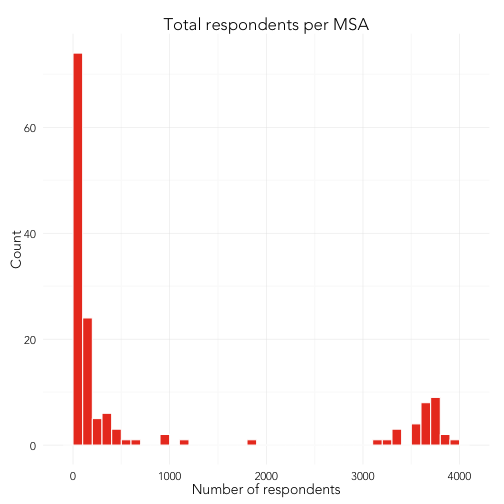
\includegraphics[scale=0.42]{compute-msa-stats-histogram-1.png}
\caption{Total respondents per MSA.}
\end{figure}

\begin{figure}
\centering 
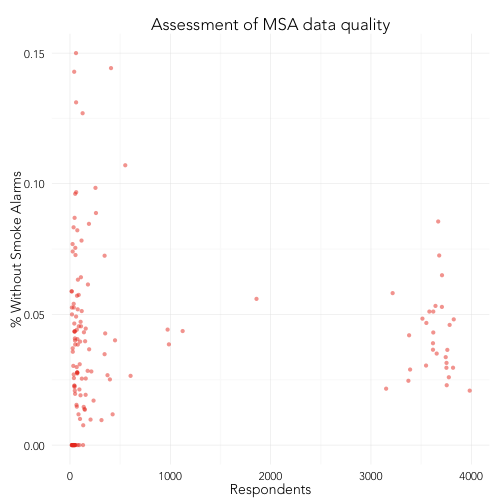
\includegraphics[scale=0.42]{compute-msa-stats-scatter-1.png}
\caption{Total respondents per MSA by percent without smoke alarms.}
\end{figure}

Since some remaining MSAs still lack sufficient data for generating reliable risk estimates, we compute a weighting factor for each MSA-level model using it's Akaike information criterion (AIC). This metric is largely a function of the sample size, but contains additional information about the model's relative strength (Figure 6).

\begin{figure}
\centering 
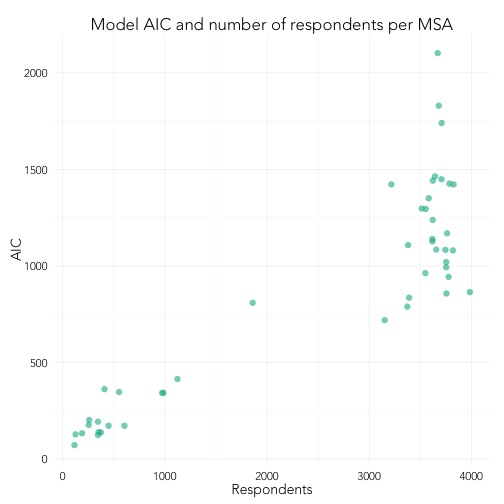
\includegraphics[scale=0.42]{estimate-msas-compare-aic-1.png}
\caption{Total respondents per MSA by model AIC.}
\end{figure}

AIC's for each model are normalized to a scale of 0.25 to 0.75 (Figure 7). We use this value to determine how much we should weight the MSA-level score when merging with a block group's national-level score.

\begin{figure}
\centering 
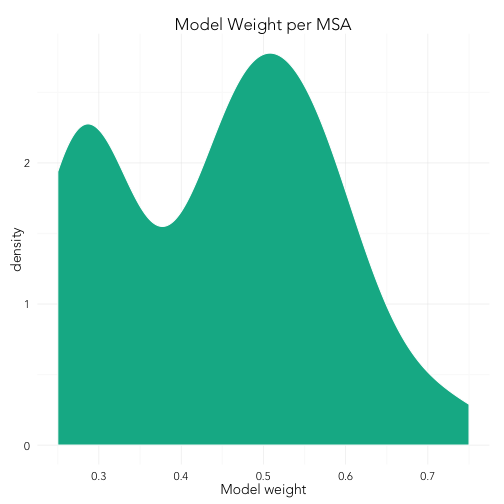
\includegraphics[scale=0.42]{estimate-msas-compare-aic-weight-1.png}
\caption{Distribution of computed MSA model weight.}}
\end{figure}

\subsubsection{Computing Risk Scores}

Overall risk scores are computed by applying the coefficients trained on the AHS to census block group-level data in the ACS. In the case a block group falls within our list of selected MSAs, we combine it's national score with it's MSA-specific score based on the MSA model's  computed weight. We then normalize this score to a scale of 0 to 1 for purposes of interpretability.

(Figure 8)
\begin{figure}
\centering 
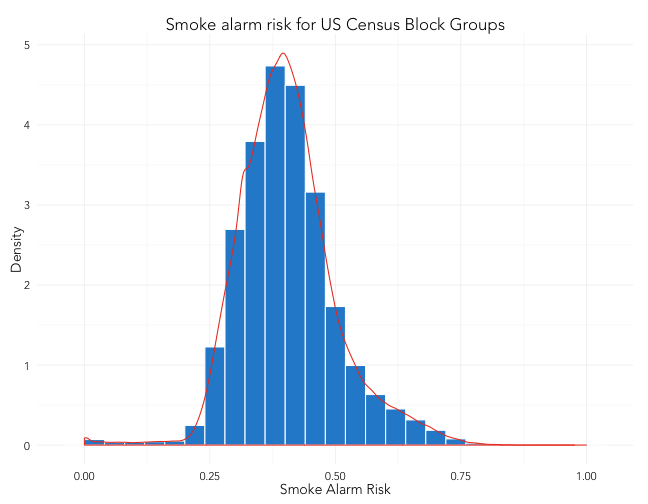
\includegraphics[scale=0.42]{compute-risk-scores-1.png}
\caption{Distribution of overall risk score per census block group.}}
\end{figure}


\subsection{TIGER Geocoder}

The Census Bureau maintains a comprehensive and deeply granular dataset of geographical features for the United States. The Topologically Integrated Geographic Encoding and Referencing (TIGER) dataset contains ESRI shapefiles that describe boundaries from the state level down to census blocks, and includes a diverse collection of geographies in between, from congressional districts to tribal reservations. By loading these files into a database capable of spatial queries, we gain the ability to situate the results of our risk model in specific areas of cities, and even on specific street blocks.

We used the Census TIGER dataset in conjunction with the PostGIS TIGER geocoder extension for the PostgreSQL database. It should be noted that our entire stack is fully open source and free to reproduce. To that end, we built a package that makes it easy for civic coders with basic skills to spin up the spatial tools that we employed for this project.\footnote{https://github.com/enigma-io/ansible-tiger-geocoder-playbook} 

\subsubsection{Block Group Geographic Join}

We first relied on the TIGER dataset to map our risk scores to specific geographical boundaries within the cities we analyzed. Each record in the ACS maps to a census block group, an area that can range in population from 600 to 3,000 citizens, and which is considered the smallest geographical entity deemed to still present valid sample data. This means that census block groups are highly variable in area. In a place like New York City, a census block group will consist of only a few blocks, whereas some areas of Alaska contain block groups that are thousands of square miles.

As mentioned above in RISK MODEL, the results of AHS are normalized over Census-designated metropolitan statistical areas. Likewise, of the total 220,740 block groups in the U.S., we generated relevant scores for the NUMBER with a population density over RATIO that fell within one of the NUMBER MSAs we deemed data-rich enough to provide reliable scores.

Finding the relevant block groups using these aforementioned tools is relatively trivial. For instance, to find block group ids that are in any given MSA, the query looks like:

\begin{lstlisting} [
           language=SQL,
           showspaces=false,
           basicstyle=\ttfamily,
           numbers=left,
           numberstyle=\tiny,
           commentstyle=\color{gray},
           breaklines=true
        ]
SELECT 
  bg_id as block_group_id
FROM 
  -- the block groups TIGER table
  tiger.bg, 
  -- the MSAs TIGER table
  -- for metro and micro areas
  tiger.cbsa
WHERE 
  -- the lsad field is 'M1' for metro 
  -- and 'M2' for micro
  tiger.cbsa.lsad='M1'
AND
  ST_Intersects(
    tiger.bg.the_geom,
    tiger.cbsa.the_geom
   )
\end{lstlisting}

\subsubsection{Address Range Resolution}

We also used the TIGER data to create a master CSV of all street blocks that fell within geographies we analyzed, coupled with their risk scores.

The TIGER data collection includes a comprehensive address ranges table that defines every street, by block, in the U.S. The 2.9m row table includes the name of a street and its left and right-side address ranges. Using geospatial querying in PostGIS, we grouped these address ranges by census block groups, and thereby joined every city block and address range to the relevant census block score in our model. 

The method employed for this was simple: for each street in the address features table, shift the line-segment defined as that street's geographical location a few meters to the left, and then a few to the right, and join these off-based line-segments to the census block geographies within which they fall. This small geographical transform for each street reduced the ambiguities that arise when streets form the border between two census block groups. In those cases, addresses on side A of a street ought to be associated with census block group A, and addresses on side B ought to be associated with census block group B. Without enacting this small transform, addresses will associate with both block groups they border, rather than the one they are actually within.

The query ultimately joins the two shifted street sides:

\begin{lstlisting} [
           language=SQL,
           showspaces=false,
           basicstyle=\ttfamily,
           numbers=left,
           numberstyle=\tiny,
           commentstyle=\color{gray},
           breaklines=true
        ]
with right_side as (
    SELECT distinct
        block_group.bg_id as block_group_id,
        right_side.fullname as street_name,
        right_side.lfromhn as from_addr,
        right_side.ltohn as to_addr
    FROM
        tiger.addrfeat as right_side,
        tiger.bg as block_group
    WHERE ST_Intersects(block_group.the_geom, right_side.the_geom)
    -- intersections of 0 length occur!
    AND St_Length(ST_Intersection(block_group.the_geom, right_side.the_geom)) > 0
    AND ST_Intersects(
        -- offset the street by a small margin
        ST_OffsetCurve(ST_LineMerge(right_side.the_geom), .00001),
        tiger.bg.the_geom
    )
)

-- identical to right_side, with offset curve set negative
with left_side as (
    SELECT distinct
        block_group.bg_id as block_group_id,
        left_side.fullname as street_name,
        left_side.lfromhn as from_addr,
        left_side.ltohn as to_addr
    FROM
        tiger.addrfeat as left_side,
        tiger.bg as block_group
    WHERE ST_Intersects(block_group.the_geom, left_side.the_geom)
    -- intersections of 0 length occur!
    AND St_Length(ST_Intersection(block_group.the_geom, left_side.the_geom)) > 0
    AND ST_Intersects(
        -- offset the street by a small margin
        ST_OffsetCurve(ST_LineMerge(left_side.the_geom), -.00001),
        tiger.bg.the_geom
    )
)

SELECT * FROM left_side
UNION ALL
SELECT * FROM right_side
\end{lstlisting}

This query fails to return distinct results when streets are simultaneously extremely curvy and very close to each other. There are a low number occurrences of this anomaly out of 14,677,020 distinct listed street ranges, 99.51\% fall within a single block group, .49\% fall within two, and only 103 blocks fall within three. Clearly there is space here to refine our work, but for practical applications, the duplication of streets within block groups are not significant enough to truly hamper outreach work on the ground.

\section{Civic Tools}

The primary purpose of this project was not analysis and research, but rather a suite of open-sourced tools that make decision-making easier for fire departments and organizations involved in fire risk mitigation. Here we outline the primary output of our efforts to date.

\subsection{Smoke Risk Portal}

All of the tools outlined below are hosted on our site, which is designed to engage directly with those who are most likely to use them. 

\subsection{Interactive Map}

We designed a granular map for every geography we analyzed so that those involved in outreach can quickly assess the risk scores for their particular locality. The map depicts census block groups for each of the 46 MSAs for which our model applies, shaded to reflect relative likelihood that an area contains households that do not have a smoke alarm.

\subsection{Address/Score CSV}

While the map offers an immediate bird's eye view of the model, we offer risk scores by address ranges as a downloadable CSV.

These CSVs are the result of joining the geospatial analysis above with our model. Each record in the CSV lists a street name, street ``start'' address and ``end'' address, a risk score, and the state and county within which the block is located, along with details about the block group associated with the street.

These CSVs were built with the intention that they would provide maximum value to local first responder and outreach communities. The data model was designed so that someone with rudimentary ability to order an Excel spreadsheet could quickly organize a list of the highest risk blocks by street name and address range for their local districts and areas of interest.

\subsection{Data Augmentation API}
While our model is built entirely from federal data, our initial work with the city of New Orleans also factored in local fire incident data. In that spirit, we built an analysis API that further enhance our risk scores when local fire incident is uploaded to an endpoint. The API accepts a CSV of local fire incident data, which must include:
\begin{itemize}
\item a latitude column (``latitude'')
\item a longitude column (``longitude'')
\item each row must represent a fire incident
\end{itemize}

It should be noted that our analysis pipeline disregards any additional features in the CSV beyond these simple requirements, thereby reducing the amount of data munging required to generate enhanced scores.

Given this information, we compute an indicator of fire incidents per census block group normalized for the included area. We also include a similar indicator which captures to percentage of "at-risk" populations (\% of people aged less than 5 or greater than 65). We then average these indicators of fire risk and at-risk population with the overall risk for residents not having smoke alarms.  This score represents our best attempt to preference populations simultaneously at risk for lacking smoke alarms and dying in home fires.

\section{Conclusion}

Prioritizing outreach efforts for fire prevention can be difficult without knowing which doors to knock on. By drawing together many different public data sets, we have developed a predictive model and analysis pipeline that increases the likelihood of finding at-risk populations.

Our goal is to provide a tool that helps fire departments and other groups work more efficiently. Local fire department outreach coordinators can combine their internal databases about local fires with geographically granular profiles for smoke alarm risk. 

This is only a first step. The City of New Orleans will soon release its first round of results following an initial pilot of this data-driven outreach program. That will provide valuable insight into ways that our model can be improved since we currently rely on federal data without the assistance of a reliable training set to verify results. 

\section{Acknowledgements}
Throughout this project, we were in close collaboration with representatives of the Red Cross and DataKind.



% The remainder of this document is concerned with showing, in
% the context of an ``actual'' document, the \LaTeX\ commands
% specifically available for denoting the structure of a
% proceedings paper, rather than with giving rigorous descriptions
% or explanations of such commands.

% \section{The {\secit Body} of The Paper}
% Typically, the body of a paper is organized
% into a hierarchical structure, with numbered or unnumbered
% headings for sections, subsections, sub-subsections, and even
% smaller sections.  The command \texttt{{\char'134}section} that
% precedes this paragraph is part of such a
% hierarchy.\footnote{This is the second footnote.  It
% starts a series of three footnotes that add nothing
% informational, but just give an idea of how footnotes work
% and look. It is a wordy one, just so you see
% how a longish one plays out.} \LaTeX\ handles the numbering
% and placement of these headings for you, when you use
% the appropriate heading commands around the titles
% of the headings.  If you want a sub-subsection or
% smaller part to be unnumbered in your output, simply append an
% asterisk to the command name.  Examples of both
% numbered and unnumbered headings will appear throughout the
% balance of this sample document.

% Because the entire article is contained in
% the \textbf{document} environment, you can indicate the
% start of a new paragraph with a blank line in your
% input file; that is why this sentence forms a separate paragraph.

% \subsection{Type Changes and {\subsecit Special} Characters}
% We have already seen several typeface changes in this sample.  You
% can indicate italicized words or phrases in your text with
% the command \texttt{{\char'134}textit}; emboldening with the
% command \texttt{{\char'134}textbf}
% and typewriter-style (for instance, for computer code) with
% \texttt{{\char'134}texttt}.  But remember, you do not
% have to indicate typestyle changes when such changes are
% part of the \textit{structural} elements of your
% article; for instance, the heading of this subsection will
% be in a sans serif\footnote{A third footnote, here.
% Let's make this a rather short one to
% see how it looks.} typeface, but that is handled by the
% document class file. Take care with the use
% of\footnote{A fourth, and last, footnote.}
% the curly braces in typeface changes; they mark
% the beginning and end of
% the text that is to be in the different typeface.

% You can use whatever symbols, accented characters, or
% non-English characters you need anywhere in your document;
% you can find a complete list of what is
% available in the \textit{\LaTeX\
% User's Guide}\cite{Lamport:LaTeX}.

% \subsection{Math Equations}
% You may want to display math equations in three distinct styles:
% inline, numbered or non-numbered display.  Each of
% the three are discussed in the next sections.

% \subsubsection{Inline (In-text) Equations}
% A formula that appears in the running text is called an
% inline or in-text formula.  It is produced by the
% \textbf{math} environment, which can be
% invoked with the usual \texttt{{\char'134}begin. . .{\char'134}end}
% construction or with the short form \texttt{\$. . .\$}. You
% can use any of the symbols and structures,
% from $\alpha$ to $\omega$, available in
% \LaTeX\cite{Lamport:LaTeX}; this section will simply show a
% few examples of in-text equations in context. Notice how
% this equation: \begin{math}\lim_{n\rightarrow \infty}x=0\end{math},
% set here in in-line math style, looks slightly different when
% set in display style.  (See next section).

% \subsubsection{Display Equations}
% A numbered display equation -- one set off by vertical space
% from the text and centered horizontally -- is produced
% by the \textbf{equation} environment. An unnumbered display
% equation is produced by the \textbf{displaymath} environment.

% Again, in either environment, you can use any of the symbols
% and structures available in \LaTeX; this section will just
% give a couple of examples of display equations in context.
% First, consider the equation, shown as an inline equation above:
% \begin{equation}\lim_{n\rightarrow \infty}x=0\end{equation}
% Notice how it is formatted somewhat differently in
% the \textbf{displaymath}
% environment.  Now, we'll enter an unnumbered equation:
% \begin{displaymath}\sum_{i=0}^{\infty} x + 1\end{displaymath}
% and follow it with another numbered equation:
% \begin{equation}\sum_{i=0}^{\infty}x_i=\int_{0}^{\pi+2} f\end{equation}
% just to demonstrate \LaTeX's able handling of numbering.

% \subsection{Citations}
% Citations to articles \cite{bowman:reasoning,
% clark:pct, braams:babel, herlihy:methodology},
% conference proceedings \cite{clark:pct} or
% books \cite{salas:calculus, Lamport:LaTeX} listed
% in the Bibliography section of your
% article will occur throughout the text of your article.
% You should use BibTeX to automatically produce this bibliography;
% you simply need to insert one of several citation commands with
% a key of the item cited in the proper location in
% the \texttt{.tex} file \cite{Lamport:LaTeX}.
% The key is a short reference you invent to uniquely
% identify each work; in this sample document, the key is
% the first author's surname and a
% word from the title.  This identifying key is included
% with each item in the \texttt{.bib} file for your article.

% The details of the construction of the \texttt{.bib} file
% are beyond the scope of this sample document, but more
% information can be found in the \textit{Author's Guide},
% and exhaustive details in the \textit{\LaTeX\ User's
% Guide}\cite{Lamport:LaTeX}.

% This article shows only the plainest form
% of the citation command, using \texttt{{\char'134}cite}.
% This is what is stipulated in the SIGS style specifications.
% No other citation format is endorsed or supported.

% \subsection{Tables}
% Because tables cannot be split across pages, the best
% placement for them is typically the top of the page
% nearest their initial cite.  To
% ensure this proper ``floating'' placement of tables, use the
% environment \textbf{table} to enclose the table's contents and
% the table caption.  The contents of the table itself must go
% in the \textbf{tabular} environment, to
% be aligned properly in rows and columns, with the desired
% horizontal and vertical rules.  Again, detailed instructions
% on \textbf{tabular} material
% is found in the \textit{\LaTeX\ User's Guide}.

% Immediately following this sentence is the point at which
% Table 1 is included in the input file; compare the
% placement of the table here with the table in the printed
% dvi output of this document.

% \begin{table}
% \centering
% \caption{Frequency of Special Characters}
% \begin{tabular}{|c|c|l|} \hline
% Non-English or Math&Frequency&Comments\\ \hline
% \O & 1 in 1,000& For Swedish names\\ \hline
% $\pi$ & 1 in 5& Common in math\\ \hline
% \$ & 4 in 5 & Used in business\\ \hline
% $\Psi^2_1$ & 1 in 40,000& Unexplained usage\\
% \hline\end{tabular}
% \end{table}

% To set a wider table, which takes up the whole width of
% the page's live area, use the environment
% \textbf{table*} to enclose the table's contents and
% the table caption.  As with a single-column table, this wide
% table will ``float" to a location deemed more desirable.
% Immediately following this sentence is the point at which
% Table 2 is included in the input file; again, it is
% instructive to compare the placement of the
% table here with the table in the printed dvi
% output of this document.


% \begin{table*}
% \centering
% \caption{Some Typical Commands}
% \begin{tabular}{|c|c|l|} \hline
% Command&A Number&Comments\\ \hline
% \texttt{{\char'134}alignauthor} & 100& Author alignment\\ \hline
% \texttt{{\char'134}numberofauthors}& 200& Author enumeration\\ \hline
% \texttt{{\char'134}table}& 300 & For tables\\ \hline
% \texttt{{\char'134}table*}& 400& For wider tables\\ \hline\end{tabular}
% \end{table*}
% % end the environment with {table*}, NOTE not {table}!

% \subsection{Figures}
% Like tables, figures cannot be split across pages; the
% best placement for them
% is typically the top or the bottom of the page nearest
% their initial cite.  To ensure this proper ``floating'' placement
% of figures, use the environment
% \textbf{figure} to enclose the figure and its caption.

% This sample document contains examples of \textbf{.eps}
% and \textbf{.ps} files to be displayable with \LaTeX.  More
% details on each of these is found in the \textit{Author's Guide}.

% \begin{figure}
% \centering
% \epsfig{file=fly.eps}
% \caption{A sample black and white graphic (.eps format).}
% \end{figure}

% \begin{figure}
% \centering
% \epsfig{file=fly.eps, height=1in, width=1in}
% \caption{A sample black and white graphic (.eps format)
% that has been resized with the \texttt{epsfig} command.}
% \end{figure}


% As was the case with tables, you may want a figure
% that spans two columns.  To do this, and still to
% ensure proper ``floating'' placement of tables, use the environment
% \textbf{figure*} to enclose the figure and its caption.
% and don't forget to end the environment with
% {figure*}, not {figure}!

% \begin{figure*}
% \centering
% \epsfig{file=flies.eps}
% \caption{A sample black and white graphic (.eps format)
% that needs to span two columns of text.}
% \end{figure*}

% Note that either {\textbf{.ps}} or {\textbf{.eps}} formats are
% used; use
% the \texttt{{\char'134}epsfig} or \texttt{{\char'134}psfig}
% commands as appropriate for the different file types.

% \begin{figure}
% \centering
% \psfig{file=rosette.ps, height=1in, width=1in,}
% \caption{A sample black and white graphic (.ps format) that has
% been resized with the \texttt{psfig} command.}
% \vskip -6pt
% \end{figure}

% \subsection{Theorem-like Constructs}
% Other common constructs that may occur in your article are
% the forms for logical constructs like theorems, axioms,
% corollaries and proofs.  There are
% two forms, one produced by the
% command \texttt{{\char'134}newtheorem} and the
% other by the command \texttt{{\char'134}newdef}; perhaps
% the clearest and easiest way to distinguish them is
% to compare the two in the output of this sample document:

% This uses the \textbf{theorem} environment, created by
% the\linebreak\texttt{{\char'134}newtheorem} command:
% \newtheorem{theorem}{Theorem}
% \begin{theorem}
% Let $f$ be continuous on $[a,b]$.  If $G$ is
% an antiderivative for $f$ on $[a,b]$, then
% \begin{displaymath}\int^b_af(t)dt = G(b) - G(a).\end{displaymath}
% \end{theorem}

% The other uses the \textbf{definition} environment, created
% by the \texttt{{\char'134}newdef} command:
% \newdef{definition}{Definition}
% \begin{definition}
% If $z$ is irrational, then by $e^z$ we mean the
% unique number which has
% logarithm $z$: \begin{displaymath}{\log e^z = z}\end{displaymath}
% \end{definition}

% Two lists of constructs that use one of these
% forms is given in the
% \textit{Author's  Guidelines}.
 
% There is one other similar construct environment, which is
% already set up
% for you; i.e. you must \textit{not} use
% a \texttt{{\char'134}newdef} command to
% create it: the \textbf{proof} environment.  Here
% is a example of its use:
% \begin{proof}
% Suppose on the contrary there exists a real number $L$ such that
% \begin{displaymath}
% \lim_{x\rightarrow\infty} \frac{f(x)}{g(x)} = L.
% \end{displaymath}
% Then
% \begin{displaymath}
% l=\lim_{x\rightarrow c} f(x)
% = \lim_{x\rightarrow c}
% \left[ g{x} \cdot \frac{f(x)}{g(x)} \right ]
% = \lim_{x\rightarrow c} g(x) \cdot \lim_{x\rightarrow c}
% \frac{f(x)}{g(x)} = 0\cdot L = 0,
% \end{displaymath}
% which contradicts our assumption that $l\neq 0$.
% \end{proof}

% Complete rules about using these environments and using the
% two different creation commands are in the
% \textit{Author's Guide}; please consult it for more
% detailed instructions.  If you need to use another construct,
% not listed therein, which you want to have the same
% formatting as the Theorem
% or the Definition\cite{salas:calculus} shown above,
% use the \texttt{{\char'134}newtheorem} or the
% \texttt{{\char'134}newdef} command,
% respectively, to create it.

% \subsection*{A {\secit Caveat} for the \TeX\ Expert}
% Because you have just been given permission to
% use the \texttt{{\char'134}newdef} command to create a
% new form, you might think you can
% use \TeX's \texttt{{\char'134}def} to create a
% new command: \textit{Please refrain from doing this!}
% Remember that your \LaTeX\ source code is primarily intended
% to create camera-ready copy, but may be converted
% to other forms -- e.g. HTML. If you inadvertently omit
% some or all of the \texttt{{\char'134}def}s recompilation will
% be, to say the least, problematic.

% \section{Conclusions}
% This paragraph will end the body of this sample document.
% Remember that you might still have Acknowledgments or
% Appendices; brief samples of these
% follow.  There is still the Bibliography to deal with; and
% we will make a disclaimer about that here: with the exception
% of the reference to the \LaTeX\ book, the citations in
% this paper are to articles which have nothing to
% do with the present subject and are used as
% examples only.
% %\end{document}  % This is where a 'short' article might terminate

% %ACKNOWLEDGMENTS are optional
% \section{Acknowledgments}
% This section is optional; it is a location for you
% to acknowledge grants, funding, editing assistance and
% what have you.  In the present case, for example, the
% authors would like to thank Gerald Murray of ACM for
% his help in codifying this \textit{Author's Guide}
% and the \textbf{.cls} and \textbf{.tex} files that it describes.

% %
% % The following two commands are all you need in the
% % initial runs of your .tex file to
% % produce the bibliography for the citations in your paper.
% \bibliographystyle{abbrv}
% \bibliography{sigproc}  % sigproc.bib is the name of the Bibliography in this case
% % You must have a proper ".bib" file
% %  and remember to run:
% % latex bibtex latex latex
% % to resolve all references
% %
% % ACM needs 'a single self-contained file'!
% %
% %APPENDICES are optional
% %\balancecolumns
% \appendix
% %Appendix A
% \section{Headings in Appendices}
% The rules about hierarchical headings discussed above for
% the body of the article are different in the appendices.
% In the \textbf{appendix} environment, the command
% \textbf{section} is used to
% indicate the start of each Appendix, with alphabetic order
% designation (i.e. the first is A, the second B, etc.) and
% a title (if you include one).  So, if you need
% hierarchical structure
% \textit{within} an Appendix, start with \textbf{subsection} as the
% highest level. Here is an outline of the body of this
% document in Appendix-appropriate form:
% \subsection{Introduction}
% \subsection{The Body of the Paper}
% \subsubsection{Type Changes and  Special Characters}
% \subsubsection{Math Equations}
% \paragraph{Inline (In-text) Equations}
% \paragraph{Display Equations}
% \subsubsection{Citations}
% \subsubsection{Tables}
% \subsubsection{Figures}
% \subsubsection{Theorem-like Constructs}
% \subsubsection*{A Caveat for the \TeX\ Expert}
% \subsection{Conclusions}
% \subsection{Acknowledgments}
% \subsection{Additional Authors}
% This section is inserted by \LaTeX; you do not insert it.
% You just add the names and information in the
% \texttt{{\char'134}additionalauthors} command at the start
% of the document.
% \subsection{References}
% Generated by bibtex from your ~.bib file.  Run latex,
% then bibtex, then latex twice (to resolve references)
% to create the ~.bbl file.  Insert that ~.bbl file into
% the .tex source file and comment out
% the command \texttt{{\char'134}thebibliography}.
% % This next section command marks the start of
% % Appendix B, and does not continue the present hierarchy
% \section{More Help for the Hardy}
% The sig-alternate.cls file itself is chock-full of succinct
% and helpful comments.  If you consider yourself a moderately
% experienced to expert user of \LaTeX, you may find reading
% it useful but please remember not to change it.
% %\balancecolumns % GM June 2007
% % That's all folks!
\end{document}
